\subsection{\texorpdfstring{THE HOMOMORPHISM \(\mathbf{E}^* \otimes_{\mathbf{A}} \mathbf{F} \to \operatorname{Hom}_{\mathbf{A}}(\mathbf{E}, \mathbf{F})\)}{THE HOMOMORPHISM \textbackslash mathbf\{E\}\^{}* \textbackslash otimes\_\{\textbackslash mathbf\{A\}\} \textbackslash mathbf\{F\} \textbackslash to \textbackslash operatorname\{Hom\}\_\{\textbackslash mathbf\{A\}\}(\textbackslash mathbf\{E\}, \textbackslash mathbf\{F\})}}

Let A, B be two rings, E a left A-module, F a left B-module and G an (A, B)-bimodule. The Z-module \(\operatorname{Hom}_{\mathbf{A}}(\mathbf{E}, \mathbf{G})\) has canonically a right B-module structure (§ 1, no. 14) such that \((u\beta)(x) = u(x)\beta\) for \(\beta \in \mathbf{B}\) , \(u \in \operatorname{Hom}_{\mathbf{A}}(\mathbf{E}, \mathbf{G})\) , \(x \in \mathbf{E}\) . On the other hand, \(\mathbf{G} \otimes_{\mathbf{B}} \mathbf{F}\) has canonically a left A-module structure (§ 3, no. 4). We shall define a canonical \(\mathbf{Z}\) -homomorphism

\[
\nu : \operatorname{Hom} _ {\mathbf {A}} (\mathrm{E}, \mathrm{G}) \otimes_ {\mathbf {B}} \mathrm{F} \rightarrow \operatorname{Hom} _ {\mathbf {A}} (\mathrm{E}, \mathrm{G} \otimes_ {\mathbf {B}} \mathrm{F}).\tag{7}
\]

To this end, we consider, for all \(y \in \mathbf{F}\) and all \(u \in \operatorname{Hom}_{\mathbf{A}}(\mathbf{E}, \mathbf{G})\) , the mapping \(\nu'(u, y): x \mapsto u(x) \otimes y\) of \(\mathbf{E}\) onto \(\mathbf{G} \otimes_{\mathbf{B}} \mathbf{F}\) . It is immediately verified that \(\nu'(u, y)\) is A-linear and that \(\nu'\) is a Z-bilinear mapping of \(\operatorname{Hom}_{\mathbf{A}}(\mathbf{E}, \mathbf{G}) \times \mathbf{F}\) into \(\operatorname{Hom}_{\mathbf{A}}(\mathbf{E}, \mathbf{G} \otimes_{\mathbf{B}} \mathbf{F})\) ; moreover, for all \(\beta \in \mathbf{B}\) , \(\nu'(u\beta, y)\) and \(\nu'(u, \beta y)\) are equal, for \((u(x)\beta) \otimes y = u(x) \otimes (\beta y)\) . We conclude (§ 3, no. 1, Proposition 1) the existence of the desired homomorphism \(\nu\) such that \(\nu(u \otimes y)\) is the A-linear mapping \(x \mapsto u(x) \otimes y\) .

It is immediately verified that, if E is an \((\mathbf{A}, (\mathbf{C}_{i}^{\prime}) ; (\mathbf{D}_{j}^{\prime}))\) -multimodule, F a \((\mathbf{B}, (\mathbf{C}_{h}^{\prime\prime}) ; (\mathbf{D}_{k}^{\prime\prime}))\) -multimodule and G an \((\mathbf{A}, (\mathbf{C}_{l}^{\prime\prime}) ; \mathbf{B}, (\mathbf{D}_{m}^{\prime\prime}))\) -multimodule, the mapping (7) is a \(((\mathbf{D}_{j}^{\prime}), (\mathbf{C}_{h}^{\prime\prime}), (\mathbf{C}_{l}^{\prime\prime}) ; (\mathbf{C}_{i}^{\prime}), (\mathbf{D}_{k}^{\prime\prime}), (\mathbf{D}_{m}^{\prime\prime}))\) -multimodule homomorphism.

PROPOSITION 2. (i) When F is a projective (resp. finitely generated projective) B-module, the canonical homomorphism (7) is injective (resp. bijective).

\begin{enumerate}
\def\labelenumi{(\roman{enumi})}
\setcounter{enumi}{1}
\item
  When E is a finitely generated projective A-module, the canonical homomorphism (7) is bijective.
\item
  Fixing E and G, for every left B-module F, we write
\end{enumerate}

\[
\mathrm{T} (\mathrm{F}) = \operatorname{Hom} _ {\mathrm{A}} (\mathrm{E}, \mathrm{G}) \otimes_ {\mathrm{B}} \mathrm{F}, \quad \mathrm{T} ^ {\prime} (\mathrm{F}) = \operatorname{Hom} _ {\mathrm{A}} (\mathrm{E}, \mathrm{G} \otimes_ {\mathrm{B}} \mathrm{F});
\]

for every left B-module homomorphism \(u: \mathbf{F} \to \mathbf{F}'\) , we write \(\mathrm{T}(u) = 1 \otimes u\) (1 here denoting the identity mapping of \(\operatorname{Hom}_{\mathbf{A}}(\mathbf{E}, \mathbf{G})\) ),

\[
\mathrm{T} ^ {\prime} (u) = \operatorname{Hom} \left(\mathrm{l} _ {\mathbb {E}}, \mathrm{l} _ {\mathbb {G}} \otimes u\right);
\]

on the other hand we write \(\nu_{F}\) instead of \(\nu\). Then we have the following lemmas:

Lemma 1. For every homomorphism \(u: \mathbf{F} \to \mathbf{F}'\) , the diagram

\[
\begin{array}{c c c} \mathrm{T(F)} & \xrightarrow {\nu_ {\mathrm{F}}} & \mathrm {T^ {\prime} (F)} \\ \mathrm{T(u)} \Big \downarrow & & \Big \downarrow \mathrm {T^ {\prime} (u)} \\ \mathrm {T(F^ {\prime})} & \xrightarrow {\nu_ {\mathrm {F^ {\prime}}}} & \mathrm {T^ {\prime} (F^ {\prime})} \end{array}\tag{8}
\]

is commutative.

The verification is immediate.

Lemma 2. Let M, N be two supplementary submodules in F and i: M → F, j: N → F the canonical injections. The diagram

\begin{enumerate}
\def\labelenumi{(\arabic{enumi})}
\setcounter{enumi}{8}
\tightlist
\item
\end{enumerate}

\pandocbounded{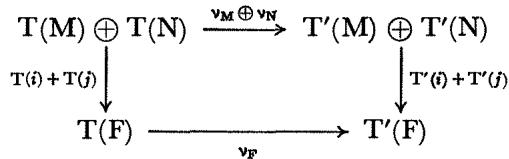
\includegraphics[keepaspectratio]{images/part002_2544dc0c.jpg}}

is commutative and the vertical arrows are bijective.

The commutativity follows from Lemma 1, the other assertions from § 1, no. 6, Corollary 2 to Proposition 6 and § 3, no. 7, Proposition 7.

Lemma 3. Under the hypotheses of Lemma 2, for \(\nu_{\mathrm{F}}\) to be injective (resp. surjective), it is necessary and sufficient that \(\nu_{\mathrm{M}}\) and \(\nu_{\mathrm{N}}\) be so.

This follows from Lemma 2 and § 1, no. 6, Corollary 1 to Proposition 6.

Then Lemma 3, together with §2, no. 2, Proposition 4, shows that it suffices to consider the case where F is a free module. But, if \((b_{\mu})\) is a basis of F, every element of \(\operatorname{Hom}_{\mathbf{A}}(\mathbf{E}, \mathbf{G}) \otimes_{\mathbf{B}} \mathbf{F}\) may then be written uniquely as \(\sum_{\mu} u_{\mu} \otimes b_{\mu}\) , where \(u_{\mu} \in \operatorname{Hom}_{\mathbf{A}}(\mathbf{E}, \mathbf{G})\) (§ 3, no. 7, Corollary 1 to Proposition 7); the image of this element under \(\nu\) is the A-linear mapping \(x \mapsto \sum_{\mu} u_{\mu}(x) \otimes b_{\mu}\) ; it cannot be zero for all \(x \in \mathbf{E}\) unless \(u_{\mu}(x) = 0\) for all \(x \in \mathbf{E}\) and all \(\mu\) , which is equivalent to saying that \(u_{\mu} = 0\) for all \(\mu\) ; hence \(\nu\) is injective. When also F admits a finite basis, Lemma 3 shows (by induction on the number of elements in the basis of F) that to prove that \(\nu\) is surjective, it suffices to do so when \(F = B_s\) ; but in this case the two sides of (7) are canonically identified with \(\operatorname{Hom}_{\mathbf{A}}(\mathbf{E}, \mathbf{G})\) (§ 3, no. 4, Proposition 4) and \(\nu\) becomes the identity.

\begin{enumerate}
\def\labelenumi{(\roman{enumi})}
\setcounter{enumi}{1}
\tightlist
\item
  To show the proposition when E is projective and finitely generated, this time we fix F and G and write, for every left A-module E,
\end{enumerate}

\[
\mathrm{T} (\mathrm{E}) = \operatorname{Hom} _ {\mathrm{A}} (\mathrm{E}, \mathrm{G}) \otimes_ {\mathrm{B}} \mathrm{F}, \quad \mathrm{T} ^ {\prime} (\mathrm{E}) = \operatorname{Hom} _ {\mathrm{A}} (\mathrm{E}, \mathrm{G} \otimes_ {\mathrm{B}} \mathrm{F})
\]

and, for every left A-module homomorphism \(v:\mathbf{E}\to\mathbf{E}^{\prime}\) ,

\[
\mathrm{T} (v) = \operatorname{Hom} (v, 1 _ {\mathbf {G}}) \otimes 1 _ {\mathbf {F}}, \quad \mathrm{T} ^ {\prime} (v) = \operatorname{Hom} (v, 1 _ {\mathbf {G}} \otimes 1 _ {\mathbf {F}});
\]

on the other hand, we write \(\nu_{E}\) instead of \(\nu\). Then we have the two lemmas:

Lemma 4. For every homomorphism \(v: \mathbf{E} \to \mathbf{E}'\) , the diagram

\[
\begin{array}{c c c} \mathrm{T} (\mathrm{E} ^ {\prime}) & \xrightarrow {\nu_ {\mathrm{E} ^ {\prime}}} & \mathrm{T} ^ {\prime} (\mathrm{E} ^ {\prime}) \\ \mathrm{T} (v) \Big \downarrow & & \Big \downarrow \mathrm{T} ^ {\prime} (v) \\ \mathrm{T} (\mathrm{E}) & \xrightarrow {\nu_ {\mathrm{E}}} & \mathrm{T} ^ {\prime} (\mathrm{E}) \end{array}\tag{10}
\]

is commutative.

Lemma 5. Let \(\mathbf{M}\) and \(\mathbf{N}\) be two supplementary submodules in \(\mathbf{E}\) and \(p: \mathbf{E} \to \mathbf{M}\) , \(q: \mathbf{E} \to \mathbf{N}\) the canonical projections. The diagram

\pandocbounded{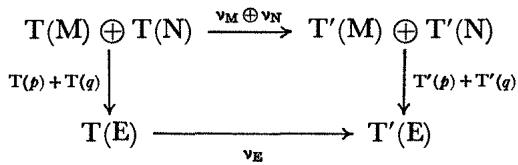
\includegraphics[keepaspectratio]{images/part002_a961576f.jpg}}

is commutative and the vertical arrows are bijective.

They are proved as Lemmas 1 and 2, taking account of § 1, no. 6, Corollary 2 to Proposition 6, § 2, no. 1, Proposition 1 and § 3, no. 7, Proposition 7.

The remainder of the proof then proceeds as in (i) and is reduced to the case where \(E = A_{s}\) ; the two sides of (7) are then canonically identified with \(G \otimes_{B} F\) and \(\nu\) becomes the identity.

In particular take B = A and G the (A, A)-bimodule \(_{s}A_{d}\) (§ 3, no. 4), so that the right A-module \(\operatorname{Hom}_{\mathbf{A}}(\mathbf{E}, _{s}\mathbf{A}_{d})\) is just the dual E* of E and \((_{s}\mathbf{A}_{d}) \otimes_{\mathbf{A}} F\) is canonically identified with F (§ 3, no. 4, Proposition 4). Homomorphism (7) then becomes a canonical Z-homomorphism

\[
\theta : \mathrm{E} ^ {*} \otimes_ {\mathrm{A}} \mathrm{F} \rightarrow \operatorname{Hom} _ {\mathrm{A}} (\mathrm{E}, \mathrm{F})\tag{11}
\]

and \(\theta (x^{*}\otimes y)\) is the linear mapping of E into F

\[
x \mapsto \langle x, x ^ {*} \rangle y.
\]

Remark (1). The characterization of projective A-modules given in §2, no. 6, Proposition 12, can also be expressed as follows: for a left A-module E to be projective, it is necessary and sufficient that the canonical homomorphism

\[
\theta_ {\mathbf {E}}: \mathrm{E} ^ {*} \otimes_ {\mathbf {A}} \mathrm{E} \rightarrow \operatorname{Hom} _ {\mathbf {A}} (\mathrm{E}, \mathrm{E}) = \operatorname{End} _ {\mathbf {A}} (\mathrm{E})
\]

be such that \(l_{E}\) belongs to the image of \(\theta_{E}\) .

COROLLARY. (i) When F is a projective (resp. finitely generated projective) module, the canonical homomorphism (11) is injective (resp. bijective).

\begin{enumerate}
\def\labelenumi{(\roman{enumi})}
\setcounter{enumi}{1}
\tightlist
\item
  When E is a finitely generated projective module, the canonical homomorphism (11) is bijective.
\end{enumerate}

Even when E and F are both finitely generated, \(\theta\) is not necessarily surjective, as is shown by the example A = Z, E = F = Z/2Z; the right hand side of (11) is non-zero but \(E^{*} = 0\) . On the other hand, examples can be given where E is free, but (11) is neither injective nor surjective (Exercise 3(b)).

When E admits a finite basis \((e_i)\) , the inverse isomorphism \(\theta^{-1}\) of \(\theta\) can be found explicitly as follows. Let \((e_i^*)\) be the dual basis of \((e_i)\) (§ 2, no. 6); for all \(u \in \operatorname{Hom}(\mathbf{E}, \mathbf{F})\) and all \(x = \sum_{i} \xi_i e_i\) with \(\xi_i \in \mathbf{A}\) ,

\[
u (x) = \sum_ {i} \xi_ {i} u (e _ {i}) = \sum_ {i} \langle x, e _ {i} ^ {*} \rangle u (e _ {i})
\]

and therefore \(u = \sum_{i} \theta(e_i^* \otimes u(e_i))\) , in other words

\[
\theta^ {- 1} (u) = \sum_ {i} e _ {i} ^ {*} \otimes u (e _ {i}).\tag{12}
\]

In particular, if further F = E, it is seen that the image under \(\theta_{E}^{-1}\) of the identity mapping \(l_{E}\) is the element \(\sum_{i} e_{i}^{*} \otimes e_{i}\) , which is therefore independent of the basis \((e_{i})\) considered in E.

Note on the other hand that when E is a finitely generated projective module the ring structure on \(\operatorname{End}_{\mathbf{A}}(\mathbf{E})\) can be transported by \(\theta_{E}^{-1}\) to \(E^{*}\otimes_{A}E\) ; it is immediately verified that, for x, y in E, \(x^{*}, y^{*}\) in \(E^{*}\) , in the ring \(\operatorname{End}_{\mathbf{A}}(\mathbf{E})\) ,

\[
\theta_ {\mathbf {E}} (x ^ {*} \otimes x) \circ \theta_ {\mathbf {E}} (y ^ {*} \otimes y) = \theta_ {\mathbf {E}} ((y ^ {*} \langle y, x ^ {*} \rangle) \otimes x).\tag{13}
\]

Remark (2). Let E be a right A-module; replacing E by E* in (11), we obtain a canonical Z-homomorphism

\[
\mathrm{E} ^ {* *} \otimes_ {\mathrm{A}} \mathrm{F} \rightarrow \operatorname{Hom} _ {\mathrm{A}} (\mathrm{E} ^ {*}, \mathrm{F}).\tag{14}
\]

On the other hand, there is a canonical A-homomorphism \(c_{E}:E\to E^{**}\) , whence there is a Z-homomorphism \(c_{E}\otimes l_{F}:E\otimes_{A}F\to E^{**}\otimes_{A}F\) ; composing the latter with the homomorphism (14), we hence obtain a canonical Z-homomorphism

\[
\theta^ {\prime}: \mathrm{E} \otimes_ {\mathrm{A}} \mathrm{F} \rightarrow \operatorname{Hom} _ {\mathrm{A}} (\mathrm{E} ^ {*}, \mathrm{F})\tag{15}
\]

such that \(\theta'(x \otimes y)\) is the linear mapping

\[
x ^ {*} \mapsto \langle x, x ^ {*} \rangle y.
\]

If E and F are projective modules, the mapping (15) is injective. For \(c_{E}\) is then injective (§2, no. 7, Corollary 4 to Proposition 13) and as F is projective, the Z-homomorphism \(c_{E} \otimes l_{F}: E \otimes_{A} F \to E^{**} \otimes_{A} F\) is also injective (§3, no. 7, Corollary 6 to Proposition 7); finally, it has been seen (Proposition 2) that the homomorphism (14) is injective, whence the conclusion.

If E is projective and finitely generated, the mapping (15) is bijective for the two mappings of which it is composed are then bijective (§ 2, no. 7, Corollary 4 to Proposition 13 and Proposition 2 above).

